\documentclass[technote]{IEEEtran}
%{{{ Packages
\usepackage[utf8]{inputenc}
\usepackage[T1]{fontenc}
\usepackage[scale=0.84]{geometry}
\usepackage[fleqn]{amsmath} 
\usepackage{amsthm,amssymb}
\usepackage{graphicx}
\usepackage{float}
\usepackage[caption=false,font=footnotesize]{subfig}
\usepackage{stfloats}
\usepackage{url}
\usepackage{caption}
\usepackage{lipsum}
\usepackage{multirow}
\usepackage{array}
\renewcommand{\arraystretch}{1.5}
\def\thesectiondis{\thesection.} 
\def\thesubsectiondis{\Alph{subsection}.} 
%}}}
%{{{ Title
\begin{document}
\begin{titlepage}
    \vspace*{\fill}
    \begin{center}
        \usefont{T1}{cmr}{m}{n}
        {\Huge CSCI-2100 Data Structures Lab}\\[0.3cm]
        {\huge Profiling Dijkstra's Algorithm}\\[0.6cm]
        {\Large Chad Chapnick}\\[0.4cm]
        {\small\today}
    \end{center}
    \vspace*{\fill}
\end{titlepage}
%}}}
\section{Introduction}

\subsection{Algorithm Complexity}

$|V| :=$ the number of vertices in the graph,  

$|E| :=$ the number of edges in G

For the linear implmentation of \texttt{minVertex}, the run time (for the worst case) 
is described by:

$$\Theta(|V|^2 + |E|)$$

where the $|E|$ term arises from the fact that we visit each edge once.

\subsection{Comparison}
%In this context, the density graph is defined as \_\_\_. 

From this we can see that if $|E| \in |V|$, 
then the upper bound for the run time is $O(|V|^2)$.


The use of a binary-heap in \texttt{minVertex} yields a 
lower time complexity on average relative to the linear implementation


%For intuition, this can be which can be though of 
%as $\Theta(|V|)$ for |V| vertices.

%the distances are stored in a -heap.

This can be broken down into two components. 
The $|V|\log|E|$ term comes from the fact that for every vertex, 
we must call the \texttt{minVertex} function.
The $|E|\log|E|$ term is the cost of adding an element to the 
heap for every edge (worst case).

The total runtime is 
$$\Theta ( (|V| + |E|) \cdot \log|E| )$$


To understand the asymptotic performance of this algorithm, 
we need to consider a few cases.
If $|E|$ is bounded above by $|V|$, (ie. $|E| \in O(|V|)$), 
then the linear implementation is $\Theta(|V|^2)$, 
and the heap implementation is $O(|V| \log |V|)$.



\section{Results}

An analysis of each implmentation was tested for 
three cases, namely: 

$$
\begin{cases}
    |E| = |V|/2 \\
    |E| = |V|  \\
    |E| = |V|^2
\end{cases}
$$

\begin{table}[!ht]
    \caption{Runtimes}
    \centering
    \begin{tabular}{|c|c|c|c|}
        \hline
        & DENSITY & LINEAR & HEAP \\ \hline
        \multirow{3}{*}{Adjacency List} 
        & $|E| \in |V|/2$ & 0.0 & 0.0 \\ [0.5ex]\cline{2-4}
        & $|E| \in |V|$ & 0.0 & 0.0 \\ \cline{2-4}
        & $|E| \in |V|^2$ & 0.0 & 0.0 \\ \hline
        \multirow{3}{*}{Adjacency Matrix}
        & $|E| \in |V|/2$ & 0.0 & 0.0 \\ \cline{2-4}
        & $|E| \in |V|$ & 0.0 & 0.0 \\ \cline{2-4}
        & $|E| \in |V|^2$ & 0.0 & 0.0 \\ \hline
    \end{tabular}
\end{table}


%\begin{figure*}[hb!]
    %\caption{Nodes of Dublin}
    %\centering
    %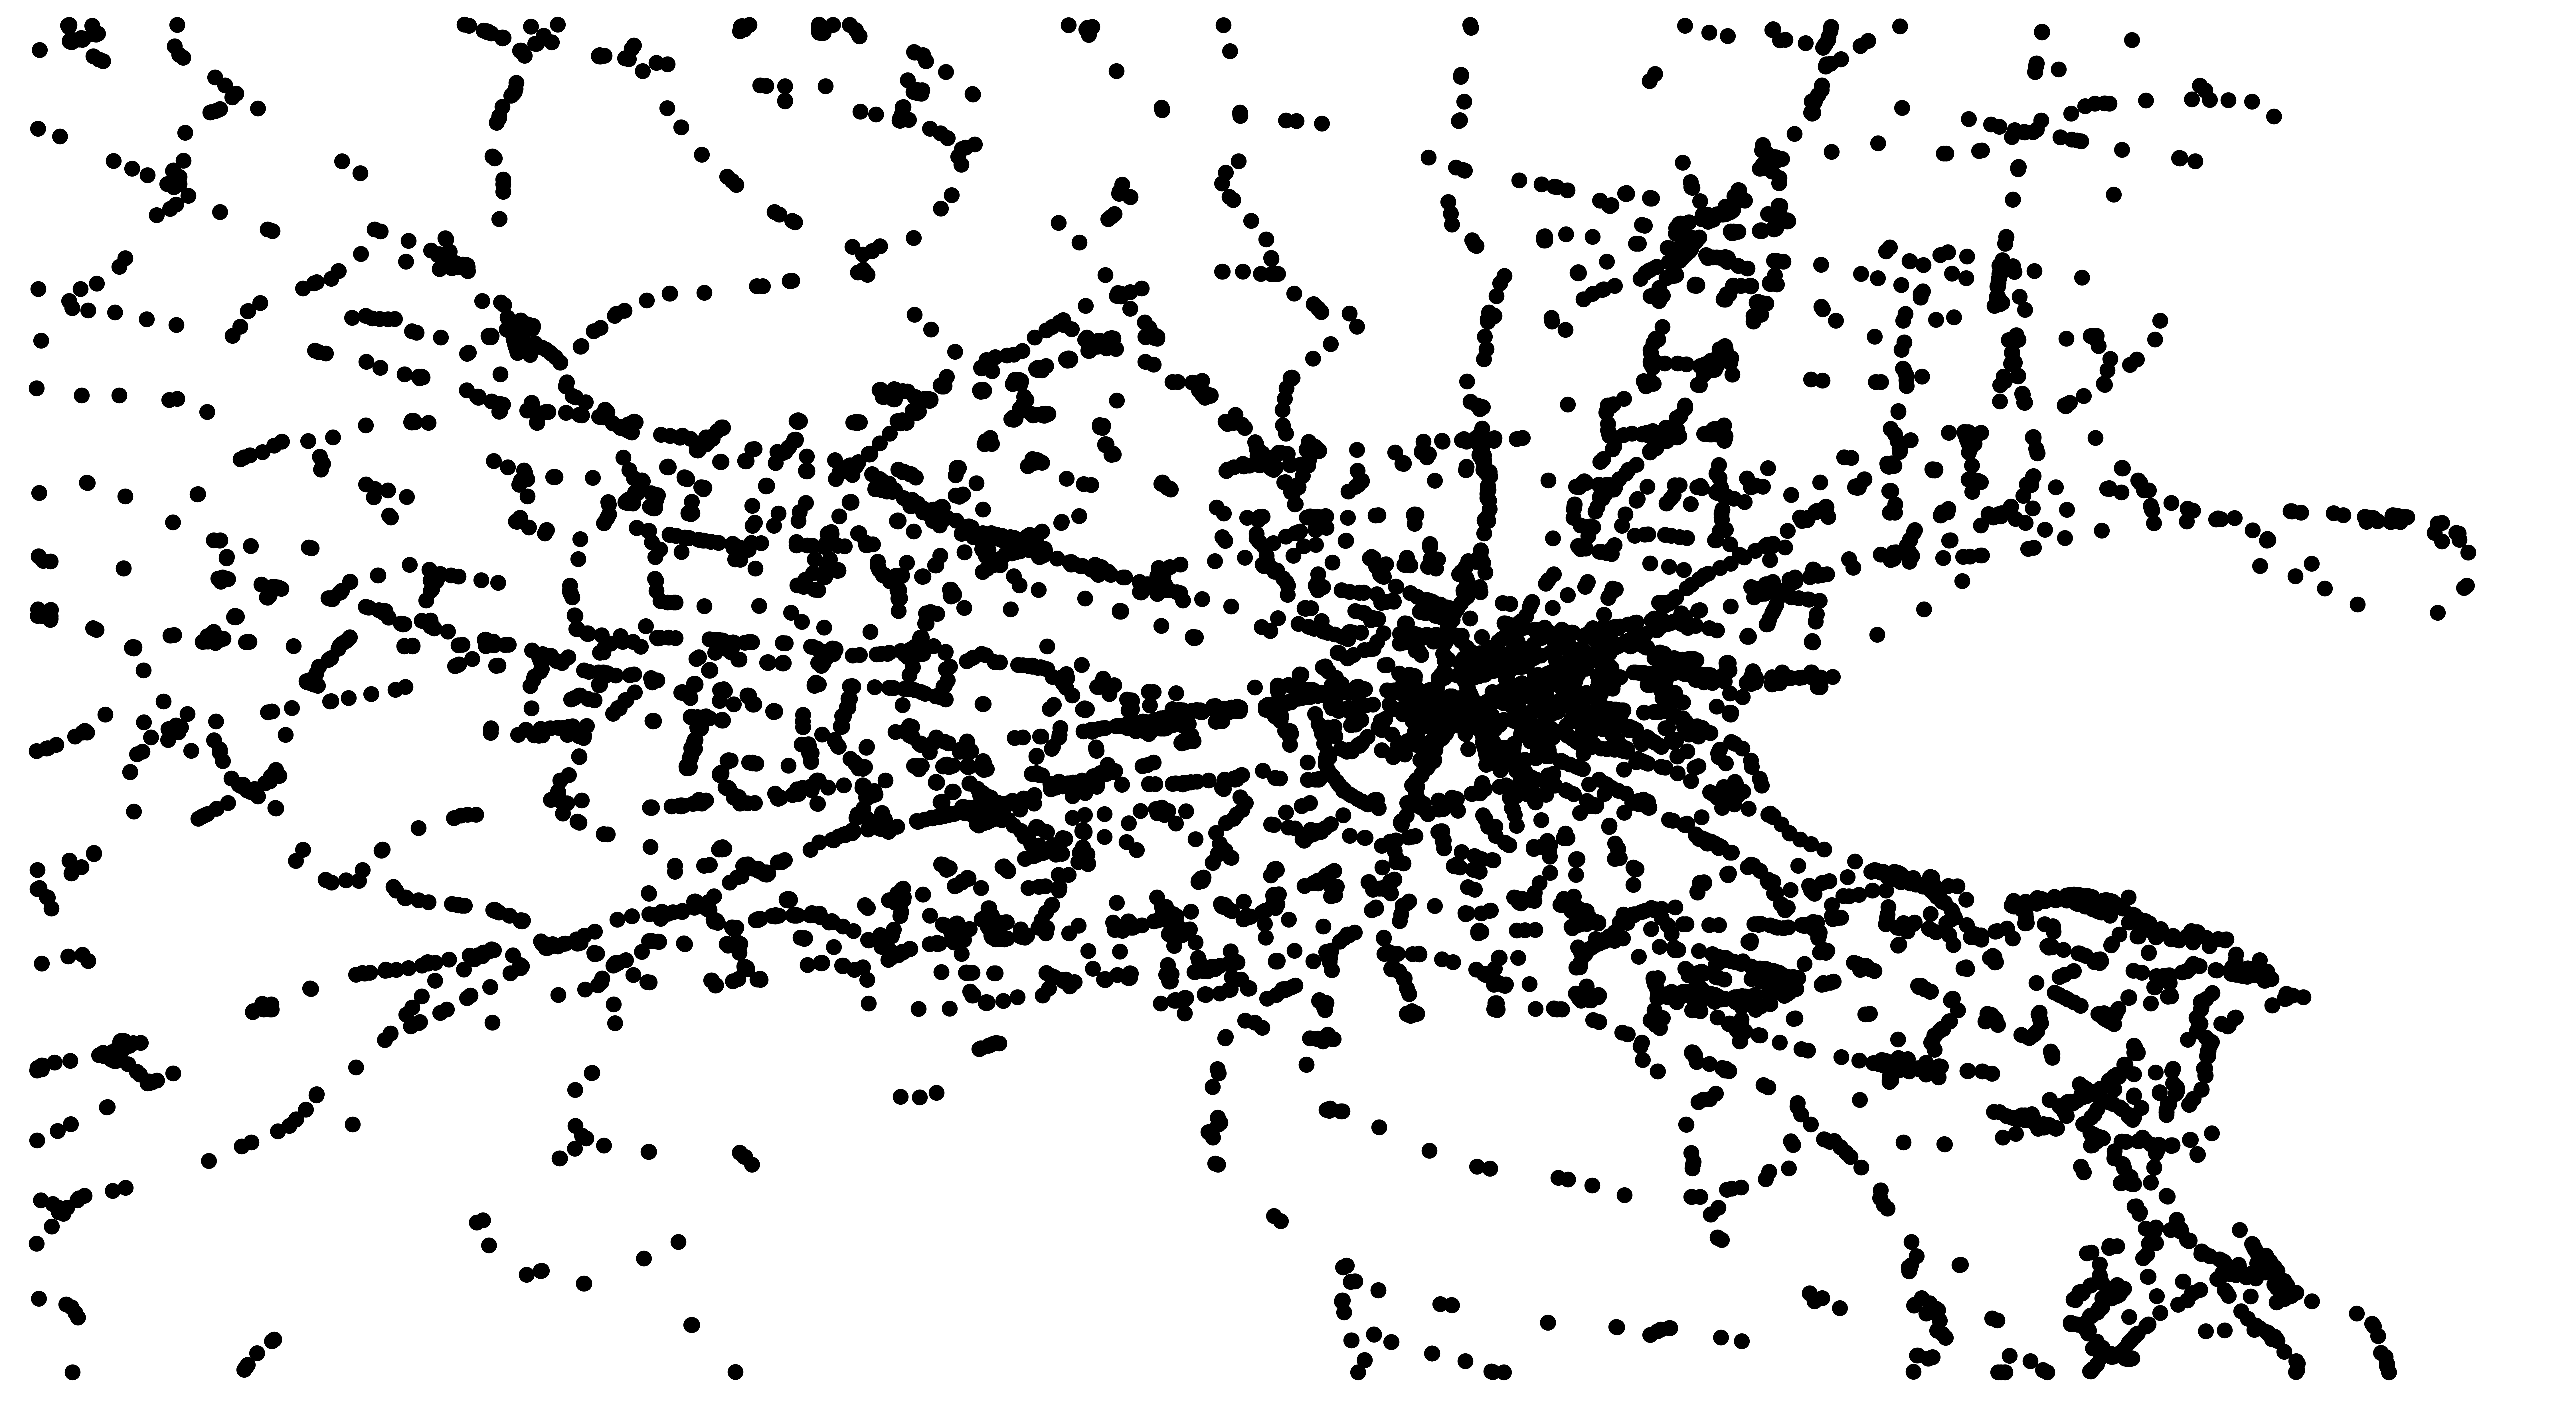
\includegraphics[width=0.75\textwidth]{scatter.png}
%\end{figure*}





\section{Conclusion}
\lipsum[1-2]
%{{{    Bibliography
\nocite{*}
\bibliographystyle{IEEEtran}
\bibliography{references.bib}
%}}}
\end{document}
